%%%%%%%%%%%%%%%%%%%%%%%%%%%%%%%%%%%%%%%%%
% Beamer Presentation
% LaTeX Template
% Version 1.0 (10/11/12)
%
% This template has been downloaded from:
% http://www.LaTeXTemplates.com
%
% License:
% CC BY-NC-SA 3.0 (http://creativecommons.org/licenses/by-nc-sa/3.0/)
%
%%%%%%%%%%%%%%%%%%%%%%%%%%%%%%%%%%%%%%%%%

%----------------------------------------------------------------------------------------
%	PACKAGES AND THEMES
%----------------------------------------------------------------------------------------

\documentclass{beamer}
\usepackage{mathtools}
\usepackage{graphicx}
\mode<presentation> {

% The Beamer class comes with a number of default slide themes
% which change the colors and layouts of slides. Below this is a list
% of all the themes, uncomment each in turn to see what they look like.

%\usetheme{default}
%\usetheme{AnnArbor}
%\usetheme{Antibes}
%\usetheme{Bergen}
%\usetheme{Berkeley}
%\usetheme{Berlin}
%\usetheme{Boadilla}
%\usetheme{CambridgeUS}
%\usetheme{Copenhagen}
%\usetheme{Darmstadt}
%\usetheme{Dresden}
%\usetheme{Frankfurt}
%\usetheme{Goettingen}
%\usetheme{Hannover}
%\usetheme{Ilmenau}
%\usetheme{JuanLesPins}
%\usetheme{Luebeck}
\usetheme{Madrid}
%\usetheme{Malmoe}
%\usetheme{Marburg}
%\usetheme{Montpellier}
%\usetheme{PaloAlto}
%\usetheme{Pittsburgh}
%\usetheme{Rochester}
%\usetheme{Singapore}
%\usetheme{Szeged}
%\usetheme{Warsaw}

% As well as themes, the Beamer class has a number of color themes
% for any slide theme. Uncomment each of these in turn to see how it
% changes the colors of your current slide theme.

%\usecolortheme{albatross}
%\usecolortheme{beaver}
%\usecolortheme{beetle}
%\usecolortheme{crane}
%\usecolortheme{dolphin}
%\usecolortheme{dove}
%\usecolortheme{fly}
%\usecolortheme{lily}
%\usecolortheme{orchid}
%\usecolortheme{rose}
%\usecolortheme{seagull}
%\usecolortheme{seahorse}
%\usecolortheme{whale}
%\usecolortheme{wolverine}

%\setbeamertemplate{footline} % To remove the footer line in all slides uncomment this line
%\setbeamertemplate{footline}[page number] % To replace the footer line in all slides with a simple slide count uncomment this line

%\setbeamertemplate{navigation symbols}{} % To remove the navigation symbols from the bottom of all slides uncomment this line
}

\usepackage{graphicx} % Allows including images
\usepackage{booktabs} % Allows the use of \toprule, \midrule and \bottomrule in tables

%----------------------------------------------------------------------------------------
%	TITLE PAGE
%----------------------------------------------------------------------------------------

\title[]{Optimized synthesized spectrum} % The short title appears at the bottom of every slide, the full title is only on the title page

\author{Jason Cao} % Your name
\institute[NYU] % Your institution as it will appear on the bottom of every slide, may be shorthand to save space
{
New York University \\ % Your institution for the title page
\medskip
\textit{jc6933@nyu.edu} % Your email address
}
\date{\today} % Date, can be changed to a custom date

\begin{document}

\begin{frame}
\titlepage % Print the title page as the first slide
\end{frame}

\begin{frame}
\frametitle{Overview} % Table of contents slide, comment this block out to remove it
\tableofcontents % Throughout your presentation, if you choose to use \section{} and \subsection{} commands, these will automatically be printed on this slide as an overview of your presentation
\end{frame}

%----------------------------------------------------------------------------------------
%	PRESENTATION SLIDES
%----------------------------------------------------------------------------------------

%------------------------------------------------
\section{Optimizing method} % Sections can be created in order to organize your presentation into discrete blocks, all sections and subsections are automatically printed in the table of contents as an overview of the talk
%------------------------------------------------

\subsection{The Cannon 2 model by Casey} % A subsection can be created just before a set of slides with a common theme to further break down your presentation into chunks

\begin{frame}
\frametitle{Details}

The model we adopt
 \[y_{jn} = v(l_n) * \theta_{jn} + e_j \]
 
 Where \(y_{jn}\) is the data for star n at wavelength pixel j. 
 
And \(v(l_n)\) is the vectorizing function. 
The input \(l_n\) is the label list of length K for star n and the  output 
\(v(l_n)\) is a vector of length D (D is bigger than K).

\( \theta_{jn}\) is a vector of length D of parameters which controlling the model at wavelength pixel j

\( e_{jn}\) is a noise draw or residual at pixel j for star n.
 

\end{frame}

%------------------------------------------------

%------------------------------------------------
\section{Optimizing method} % Sections can be created in order to organize your presentation into discrete blocks, all sections and subsections are automatically printed in the table of contents as an overview of the talk
%------------------------------------------------

\subsection{Optimize the spectrum} % A subsection can be created just before a set of slides with a common theme to further break down your presentation into chunks

\begin{frame}
\frametitle{Details}

After training the model, \(v(l_n)\) and \(\theta_{jn}\) are available.

\(y_{jn}^synthesized\) is the synthesized spectrum data for star n at pixel j by Casey's 
Cannon 2.

\(y_{jn}^synthesized=v(l_n^inferred)*\theta_{jn}\) and \(l_n^inferred\) is the 
inferred labels from Casey's Cannon 2.
 
Get \(y_{j,n-1}^synthesized\) and \(y_{j,n+1}^synthesized\) by moving the synthesized spectrum one pixel left and one pixel right.

Fit the spectrum linearly by using 
\[y_{j,n}^optimized = a*y_{j,n-1}^synthesized + b*y_{j,n}^synthesized+c*y_{j,n+1}^synthesized\]
And a+b+c should be 1



\end{frame}

%------------------------------------------------
\section{Plot}
%------------------------------------------------

\begin{frame}
\frametitle{Table}
\begin{table}
\begin{tabular}{l l l}
\toprule
\textbf{Treatments} & \textbf{Response 1} & \textbf{Response 2}\\
\midrule
Treatment 1 & 0.0003262 & 0.562 \\
Treatment 2 & 0.0015681 & 0.910 \\
Treatment 3 & 0.0009271 & 0.296 \\
\bottomrule
\end{tabular}
\caption{Table caption}
\end{table}
\end{frame}

%------------------------------------------------

%------------------------------------------------

%------------------------------------------------
\section{Plot} % Sections can be created in order to organize your presentation into discrete blocks, all sections and subsections are automatically printed in the table of contents as an overview of the talk
%------------------------------------------------

\subsection{Labels} % A subsection can be created just before a set of slides with a common theme to further break down your presentation into chunks

\begin{frame}
\frametitle{Details}

After training the model, \(v(l_n)\) and \(\theta_{jn}\) are available.

\(y_{jn}^observed\) is blue


\(y_{jn}^inferred\) is green


\(y_{jn}^synthesized\) is red



\end{frame}

%------------------------------------------------



%------------------------------------------------
\section{Plot} % Sections can be created in order to organize your presentation into discrete blocks, all sections and subsections are automatically printed in the table of contents as an overview of the talk
%------------------------------------------------

\subsection{Compare spectrum} % A subsection can be created just before a set of slides with a common theme to further break down your presentation into chunks

\begin{frame}
\frametitle{Details}
 
Compare the spectrum: a+b+c=0.984  (a,b,c)=(0.537,0.114,0.333 )


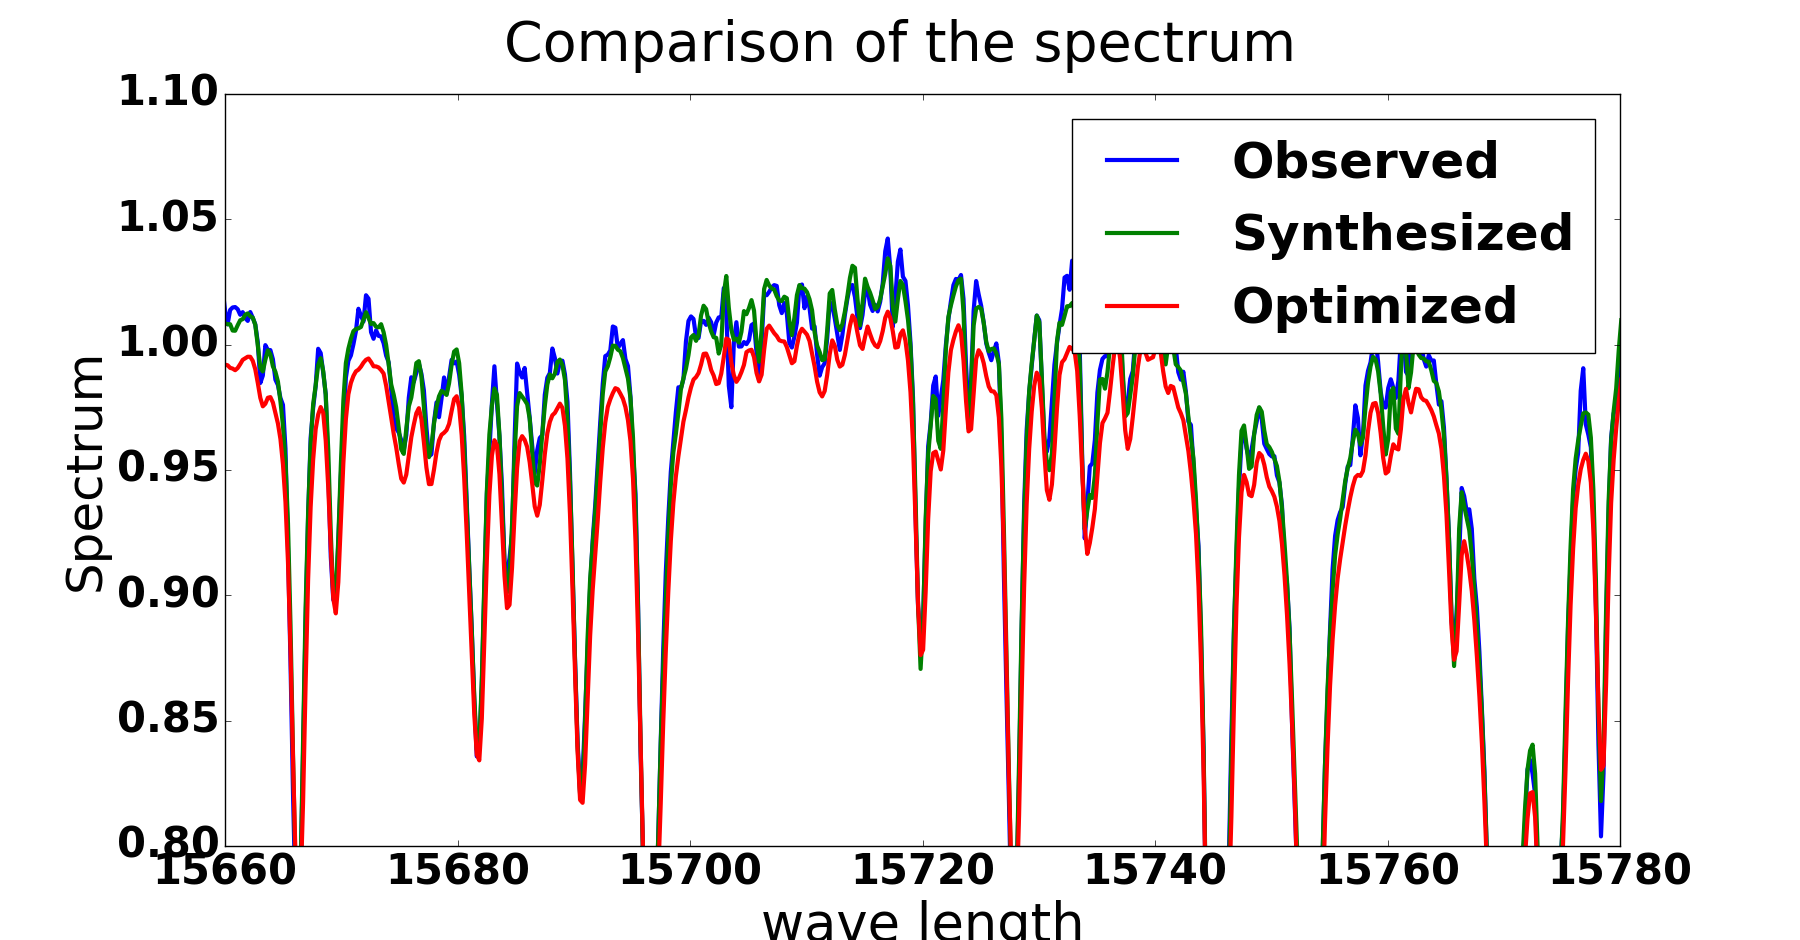
\includegraphics[width=100mm]{figure_1.png}




\end{frame}

%------------------------------------------------

%------------------------------------------------
\section{Plot} % Sections can be created in order to organize your presentation into discrete blocks, all sections and subsections are automatically printed in the table of contents as an overview of the talk
%------------------------------------------------

\subsection{Compare Chi-Square} % A subsection can be created just before a set of slides with a common theme to further break down your presentation into chunks

\begin{frame}
\frametitle{Details}
 
The chi-squared plot

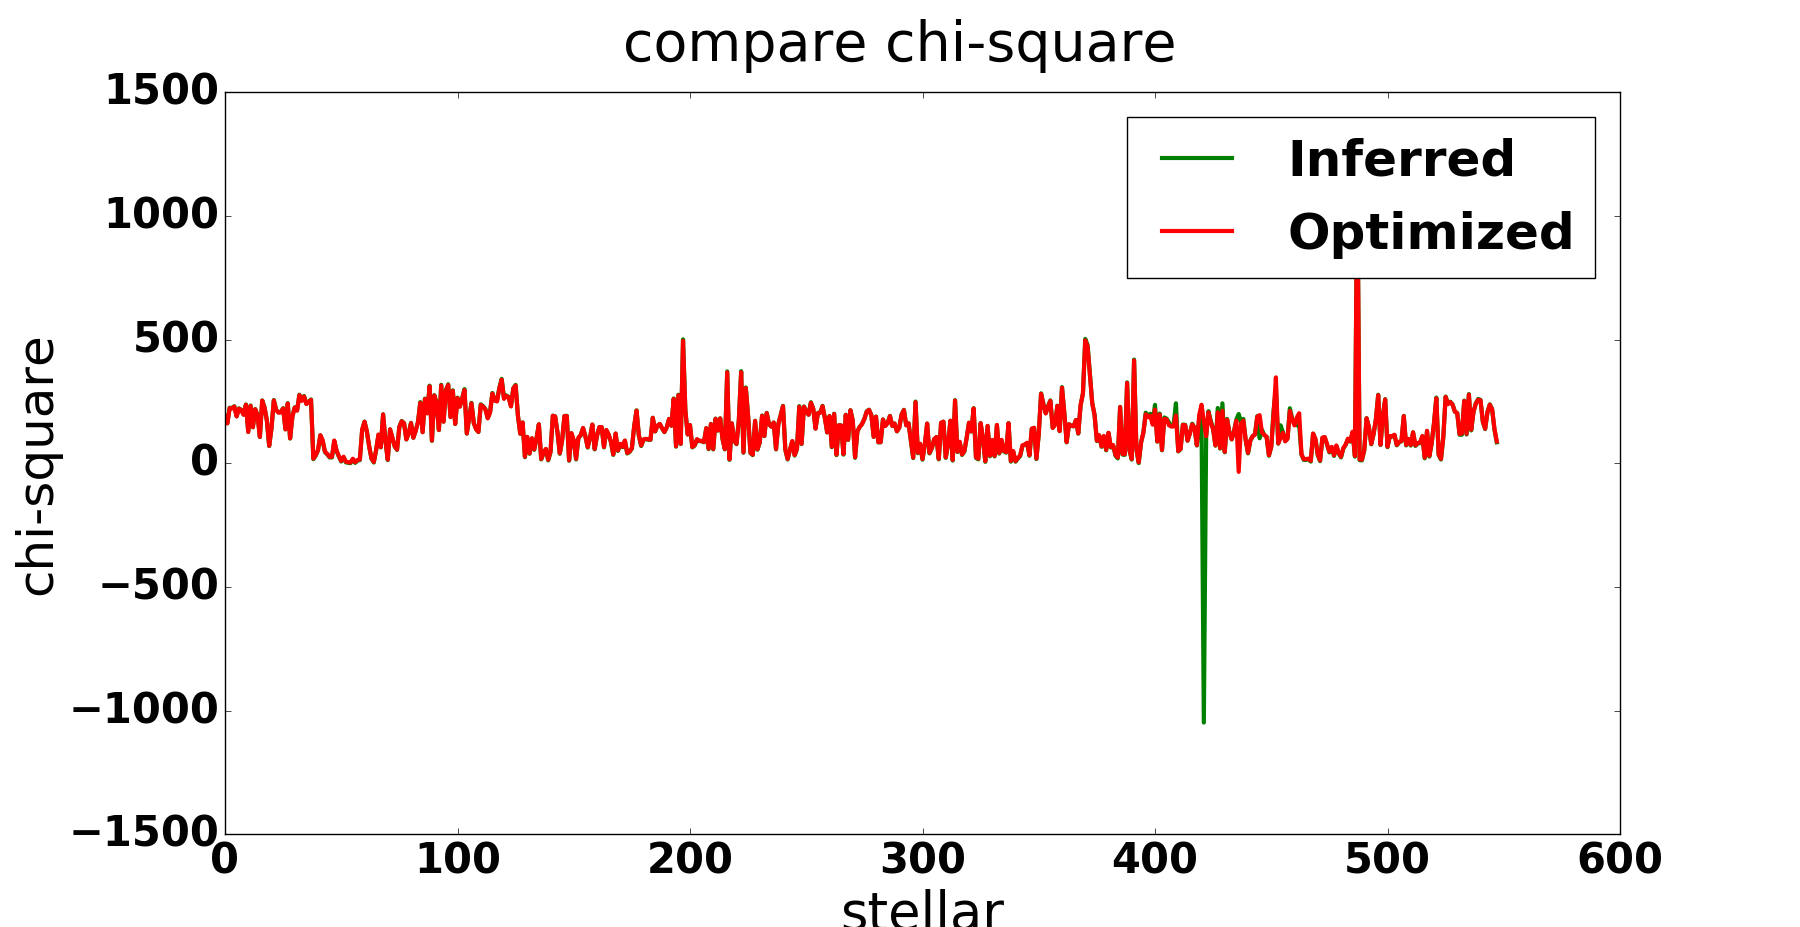
\includegraphics[width=110mm]{parameter.png}


\end{frame}



\begin{frame}
\Huge{\centerline{The End}}
\end{frame}

%----------------------------------------------------------------------------------------

\end{document} 